\section{Introduction}
\label{AABB_tree_section_intro}

The AABB tree component offers a static data structure and algorithms to perform efficient intersection and projection of 3D queries against a large set of 3D geometric objects. Examples of intersection queries include line objects (rays, lines or segments) against sets of triangles, and plane objects (planes or triangles) against sets of segments. A common example of projection query is to find the closest point from a point query to a set of triangles.

More generally, the set of geometric objects stored in the data structure may be queried for intersection detection, intersection computation and distance queries with any type of query, provided that the corresponding intersection and distance predicates and constructors are implemented in the traits class. 

The data structure takes as input an iterator range of geometric primitives, where each primitive wraps both one input geometric object (so-called datum) and one reference id to this object (e.g., wraps a 3D triangle and a face handle of a polyhedral surface). From these primitives a hierarchy of axis-aligned bounding boxes (AABBs) is constructed and used to speed up intersection and distance queries (see Figure~\ref{fig:AABB-tree-shark}). 

\begin{center}
    \label{fig:AABB-tree-shark}
    \begin{ccTexOnly}
      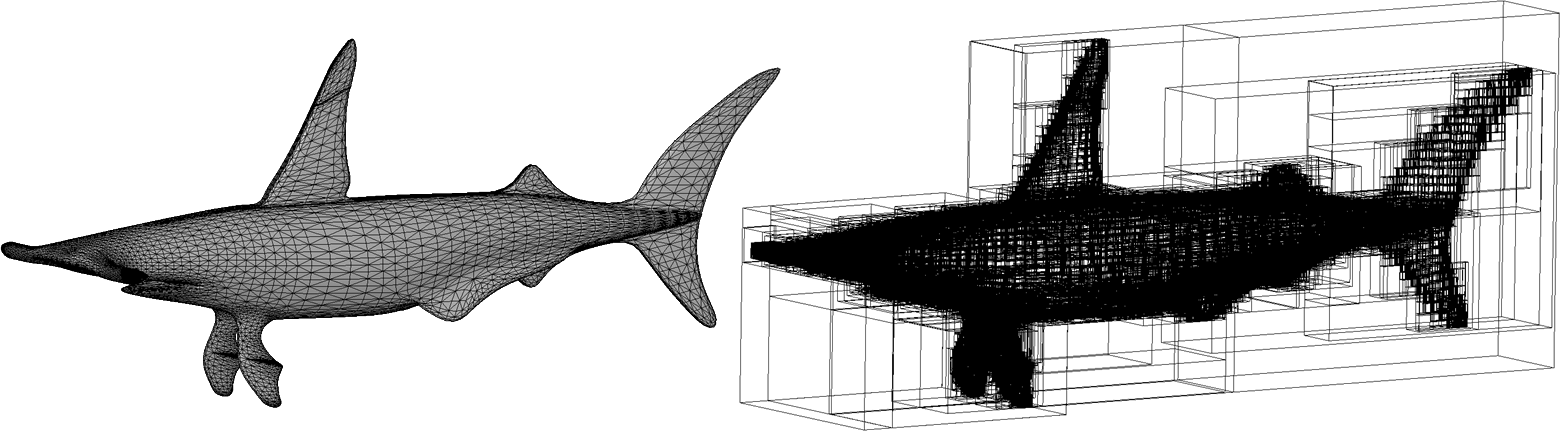
\includegraphics[width=1.0\textwidth]{AABB_tree/shark}
    \end{ccTexOnly}
    \begin{ccHtmlOnly}
        <img width="90%" border=0 src="./shark.png"><P>
    \end{ccHtmlOnly}
    \begin{figure}[h]
        \caption{AABB tree.
                 Left: surface triangle mesh of a shark.
                 Right: AABB tree constructed.}
    \end{figure}
\end{center}
